\chapter{Tools}

In \cref{tab:softwaretools}, the tools used are listed. 
Additionally, in \cref{tab:softwaretoolslinks}, the links to non-obvious tools are documented.

\begin{table}[h!]
    \centering
    \begin{tabularx}{\textwidth}{|l|l|X|}
        \hline
        \textbf{Tool Name} & \textbf{Version} & \textbf{Description}   \\ \hline
        Visual Studio Code & 1.83 & Code editor with support for debugging, syntax highlighting, and extensions. \\ \hline
        Git & 2.42 & Version control system for tracking code changes. \\ \hline
        Raspberry Pi OS & 2024-11-13 & Operating system used on the Raspberry Pi. \\ \hline
        Python & 3.11.6 & Collection of open-source Python frameworks for data science-related tasks. \\ \hline
        draw.io & 26.0.4 & Free drawing tool to create diagrams. \\ \hline
        \acrlong{dfc} & 3.29.0 & \acrlong{dfc} from Hailo to compile neural networks. \\ \hline
        Hailo firmware & 4.17.0 & Hailo firmware for using the Hailo hardware accelerator with the Raspberry Pi. \\ \hline
        Hailonet & 1.0 & A part of HailoRT to use GStreamer elements on Raspberry Pi. \\ \hline
        Hailotools & 3.29.0 & TAPPAS GStreamer elements. \\ \hline
        ONNX modifier & a761e0b & Tool to cut and edit ONNX graphs. \\ \hline
    \end{tabularx}
    \caption{Software tools used.}
    \label{tab:softwaretools}
\end{table}

\begin{table}[h!]
    \centering
    \begin{tabularx}{\textwidth}{|l|X|}
        \hline
        \textbf{Description} & \textbf{Link} \\ \hline
        Hailo Raspberry Pi & \url{https://github.com/hailo-ai/hailo-rpi5-examples/blob/main/doc/install-raspberry-pi5.md} \\ \hline
        ONNX modifier & \url{https://github.com/ZhangGe6/onnx-modifier} \\ \hline
        \acrlong{dfc} & \url{https://hailo.ai/developer-zone/software-downloads/} \\ \hline
    \end{tabularx}
    \caption{Links to tools.}
    \label{tab:softwaretoolslinks}
\end{table}

\begin{table}[h!]
    \centering
    \begin{tabularx}{\textwidth}{|l|l|X|}
        \hline
        \textbf{Repo Name} & \textbf{Git Hash} & \textbf{Description}   \\ \hline
        Documentation & a761e0b & \LaTeX code. \\ \hline
        PC Code & a761e0b & Code to get, translate, and evaluate models. \\ \hline
        Hailo Code & 8d7385a & Code to evaluate models on Hailo. \\ \hline
    \end{tabularx}
    \caption{Used Git repositories.}
    \label{tab:git}
\end{table}

\begin{table}[h!]
    \centering
    \begin{tabularx}{\textwidth}{|l|X|}
        \hline
        \textbf{Description} & \textbf{Link} \\ \hline
        Documentation & \url{https://github.com/xXAlgoorXx/Projektarbeit1_doku} \\ \hline
        Raspberry Pi & \url{https://github.com/xXAlgoorXx/EvalRaspi} \\ \hline
        PC & \url{https://github.com/xXAlgoorXx/ProjWork1_DFC} \\ \hline
    \end{tabularx}
    \caption{Links to Git repositories.}
    \label{tab:gitlinks}
\end{table}


\begin{figure}
    \centering
    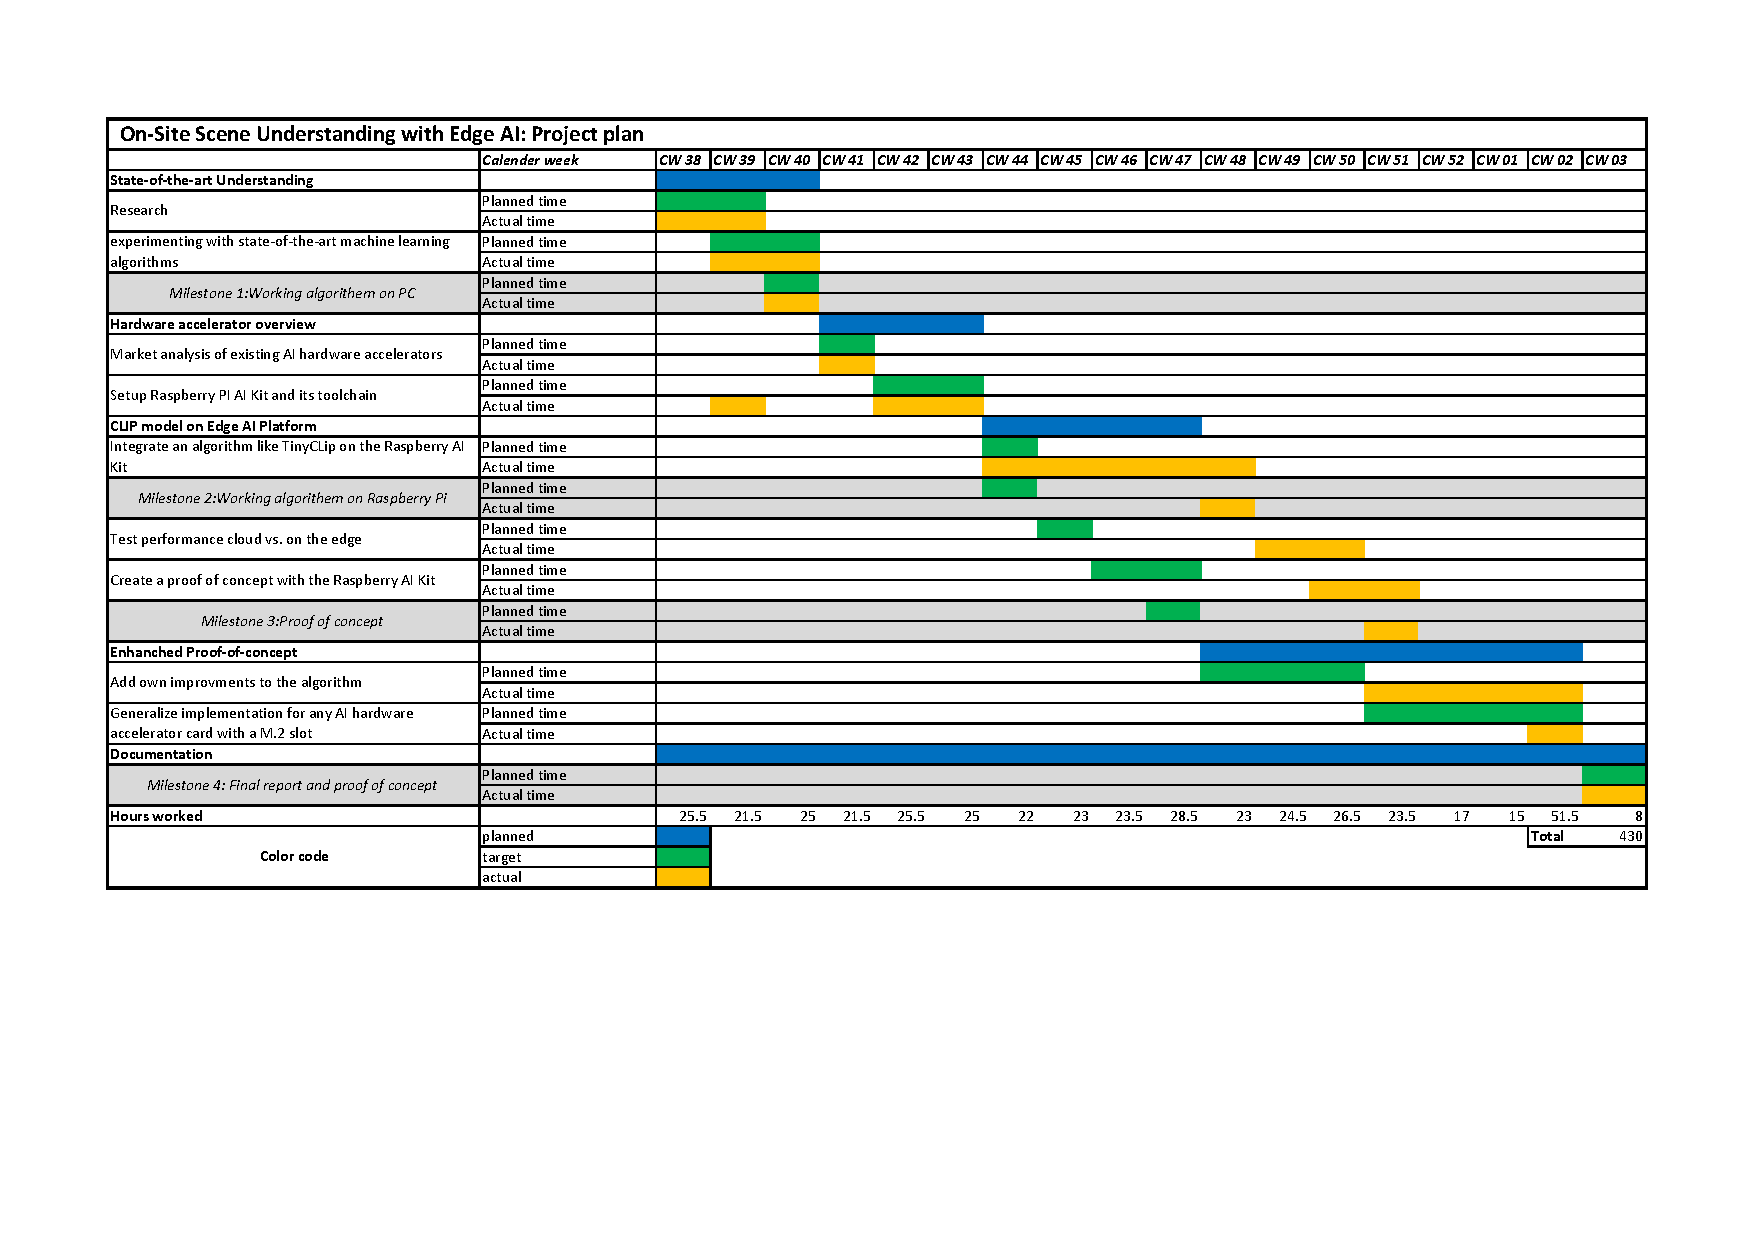
\includegraphics[angle = 90,height = \textheight]{Images/appendix/timetable_Lukas_cut.pdf}
    \caption{timetable}
\end{figure}